\subsection{Unpacking}
The \lucid cameras are capable of
\begin{figure}
    \centering
    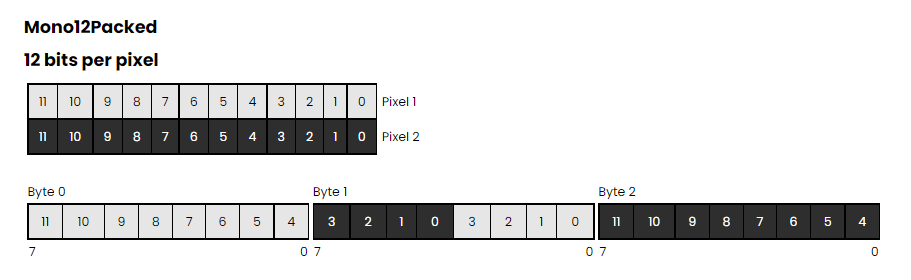
\includegraphics[width=\textwidth]{figures/Mono12Packed.png}
    \caption{Bit layout of the \cite{fisherRe15406LUT2023}}
    \label{fig:mono12packed}
\end{figure}

\begin{listing}[H]
    \begin{minted}{cuda}
        template <int width, int width_in>
        __device__ __forceinline__ void unpack10(__half2 *work_row, 
                                                 const unsigned int *img_row,
                                                 int tx) {
            __half2 *const out = &work_row[tx * 8 + 2];
        
            if (tx * 5 < width_in) {
                unsigned int buf_a, buf_b;
                buf_a = img_row[tx * 5];
                buf_b = img_row[tx * 5 + 1];
                out[0] = __halves2half2(buf_a & 0b1111111111, 
                                        buf_a >> 10 & 0b1111111111);
                out[1] = __halves2half2(buf_a >> 20 & 0b1111111111,
                                        buf_a >> 30 & 0b11 | (buf_b & 0b11111111) << 2);
        
                buf_a = img_row[tx * 5 + 2];
                out[2] = __halves2half2(buf_b >> 8 & 0b1111111111, 
                                        buf_b >> 18 & 0b1111111111);
                out[3] = __halves2half2(buf_b >> 28 & 0b1111 | (buf_a & 0b111111) << 4,
                                        buf_a >> 6 & 0b1111111111);

                buf_b = img_row[tx * 5 + 3];
                out[4] = __halves2half2(buf_a >> 16 & 0b1111111111,
                                        buf_a >> 26 & 0b111111 | (buf_b & 0b1111) << 6);
                out[5] = __halves2half2(buf_b >> 4 & 0b1111111111, 
                                        buf_b >> 14 & 0b1111111111);
        
                buf_a = img_row[tx * 5 + 4];
                out[6] = __halves2half2(buf_b >> 24 & 0b11111111 | (buf_a & 0b11) << 8,
                                        buf_a >> 2 & 0b1111111111);
                out[7] = __halves2half2(buf_a >> 12 & 0b1111111111, 
                                        buf_a >> 22 & 0b1111111111);
            }
            if (tx < 2) {
                work_row[tx] = work_row[tx + 2];
            } else if (tx >= width - 2 && tx < width) {
                work_row[tx + 4] = work_row[tx + 2];
            }
        }
    \end{minted}
    \caption{Bit unpacking in \cuda}
\end{listing}